\documentclass[12pt]{article}
\usepackage{amsmath,amsfonts,fullpage,amsthm,graphicx}

\newtheorem*{theorem}{Theorem}
\newtheorem*{fact}{Fact}
\newtheorem*{goal}{Goal}
\newtheorem*{idea}{Idea}
\newtheorem*{defn}{Definition}
\newtheorem*{ex}{Example}

%Style section
%\setlength{\textheight}{10in}
%\setlength{\textwidth}{7in}
%\hoffset=-0.75in
 \pagestyle{plain}
% \setlength{\topmargin}{0in}
% \setlength{\headsep}{0in}
% \setlength{\oddsidemargin}{0in}
% \setlength{\evensidemargin}{0in}

\begin{document}


\pagestyle{empty} %use this to get rid of page numbers

\noindent
{Math 166 \hskip 1.5 truein  Names:\ \hrulefill}

\noindent
%\vskip 0.3truein
%\bigskip
%\noindent
{Area Activity}

\noindent ~ \hskip 3.5 truein  Section Number:\ \hrulefill
\medskip

\begin{goal} \rm
Use the integral to find the area of various regions. In each problem, be sure to draw a graph of the functions.
\end{goal}
%\smallskip

\begin{enumerate}
%\setcounter{enumi}{-1}

\item Find the area enclosed between $y=\sin(x)$, $y=\cos(x)$, $x=0$, and $x=\pi$.
%over the interval $[0,\pi]$.

\vspace{3.5in}

\item Find the area of the region bounded by $y=e^x$, $y=14-e^x$, and the $y$-axis.



\vspace{3.5in}

\item Find the area of the region enclosed between $x=y^2-5$ and $x=3-y^2$. 

\vspace{3.5in}

\item Sketch a region whose area is represented by $\displaystyle\int_{-\sqrt{2}/2}^{\sqrt{2}/2} \left(\sqrt{1-x^2} - |x|\right) \ dx$ and evaluate using geometry.

\newpage

\item A sketch of the functions $f(x)$ and $g(x)$ is drawn below:
\begin{center}
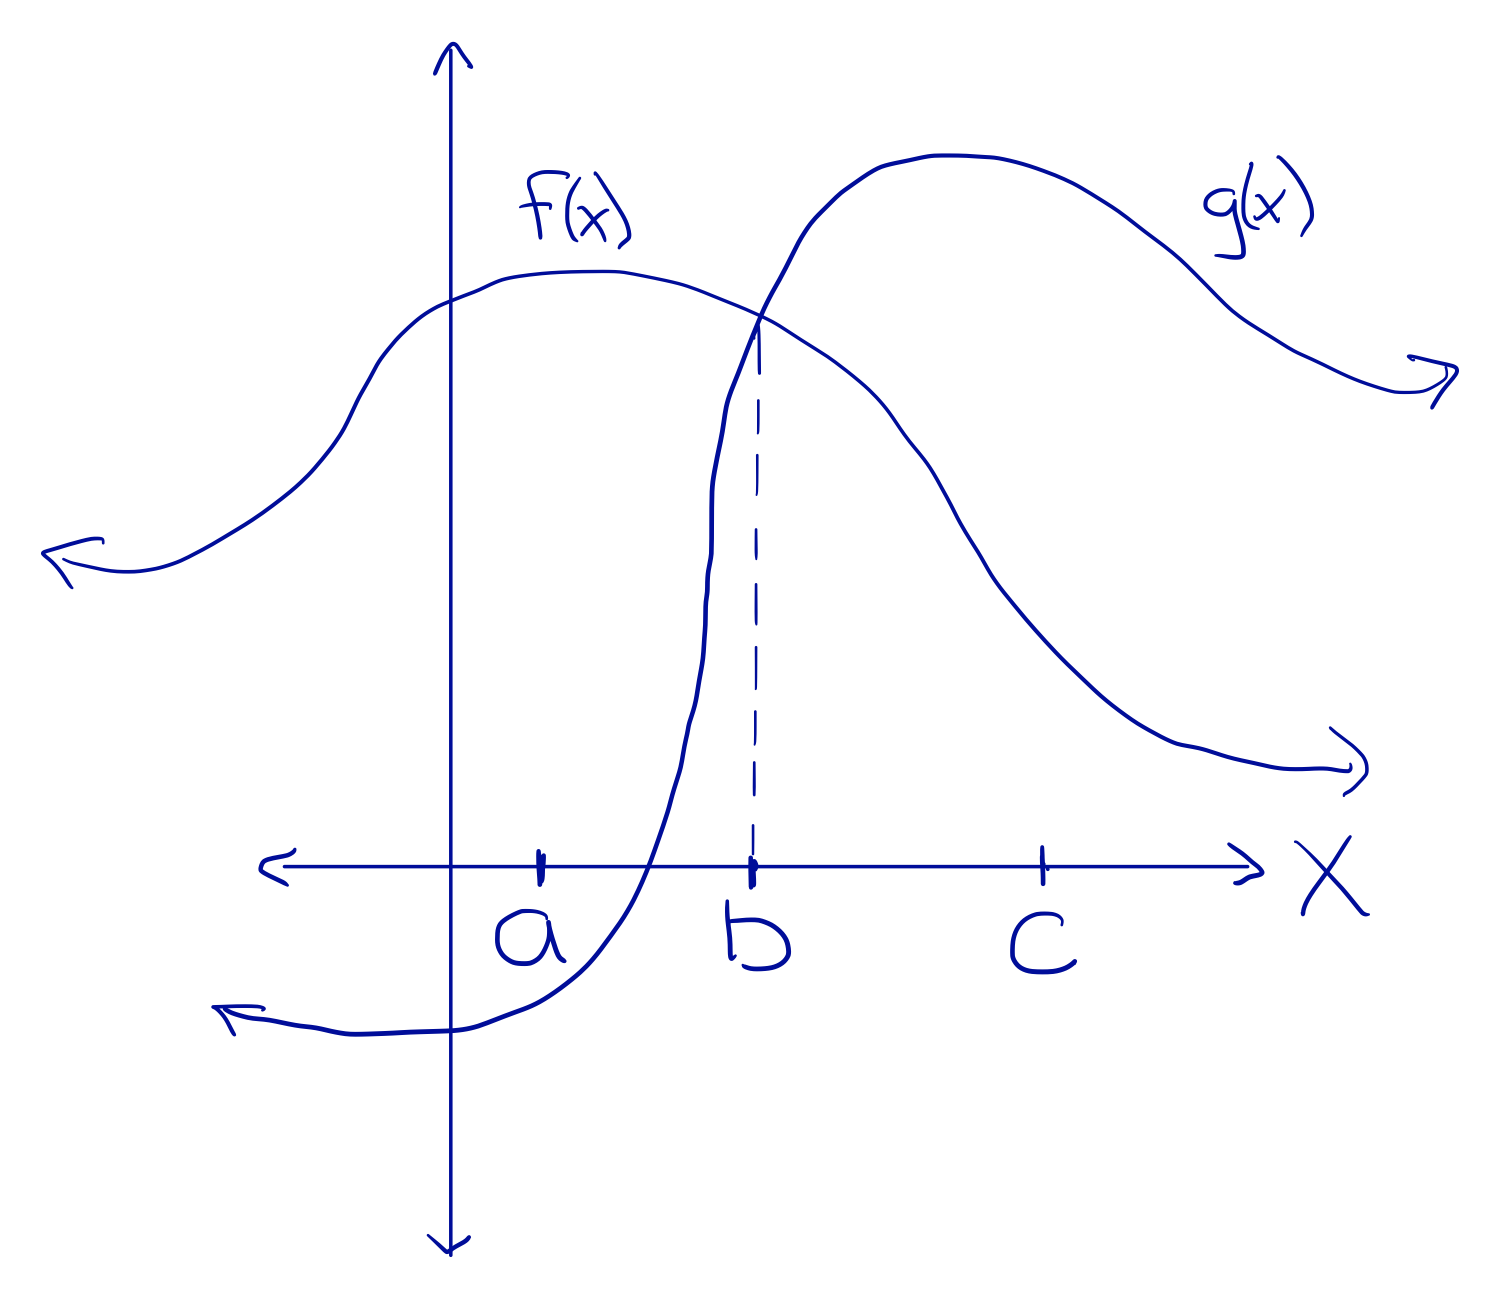
\includegraphics[width=0.6\textwidth]{AreaDrawing.png}
\end{center}
Here, $\displaystyle \int_a^b |f(x) - g(x)| \, dx = 8$ and $\displaystyle \int_b^c |f(x) - g(x)| \, dx = 12$. 
\begin{enumerate}
\item What is $\displaystyle \int_a^c (f(x) - g(x)) \, dx$?
\vfill
\item What is $\displaystyle \int_a^c |f(x) - g(x)| \, dx$?
\vfill
\end{enumerate}
\end{enumerate} 

\end{document}
